\section{BenutzerInnen-Anwendung}

Bei der BenutzerInnen-Anwendung handelt es sich um die Ansteuerung eines Moving Heads mittels  Digital Multiplex (DMX) Protokoll.  

\subsection{Grundlegender Aufbau des DMX Protokolls}
Es gibt mehrere verschiedene Spezifikationen für das DMX Protokoll. Im folgenden wird eine dieser unterschiedlichen Spezifikation erläutert und anschließend zu Vergleichszwecken verwendet. Abbildung \ref{fig:DMX-512-Protocol} dient zur Veranschaulichung des DMX-512 Protokolls. 

% http://mc.mikrocontroller.com/de/dmx512.php
% TODO: add reference to this webside

\begin{figure}[H]
	
\includegraphics[scale=0.60]{chapters/userapplication/figures/todo}
	\caption{DMX Protokoll}
	\label{fig:DMX-512-Protocol}
\end{figure}

Tabelle \ref{table:DMX-512-Protocol} beschreibt die einzeln nummerierten Markierungen aus Abbildung \ref{fig:DMX-512-Protocol}.

\begin{table}[H]
\begin{tabular}{p{1.5cm} | p{6.5cm} | p{1cm} | p{1cm} | p{1cm} | p{1cm}}
  \textbf{Nummer} & \textbf{Signalname} & \textbf{Min.} & \textbf{Typ.} & \textbf{Max.} & \textbf{Einheit} \\ 
  \hline
  1 & Reset & 88.0 & 88.0 & - & $\mu$s \\
  2 & Mark zwischen Reset- und Startbyte & 8.0 & - & 1 s & $\mu$s \\
  3 & Frame-Zeit & 43.12 & 44.0 & 44.48 & $\mu$s \\
  4 & Startbit & 3.92 & 4.0 & 4.08 & $\mu$s \\
  5 & LSB (niederwertigstes Datenbit) & 3.92 & 4.0 & 4.08 & $\mu$s \\
  6 & MSB (höchstwertigstes Datenbit) & 3.92 & 4.0 & 4.08 & $\mu$s \\
  7 & Stopbit & 3.92 & 4.0 & 4.08 & $\mu$s \\
  8 & Mark zwischen Frames (Interdigit) & 0 & 0 & 1.0 & s \\
  9 & Mark zwischen Paketen & 0 & 0 & 1.0 & s \\
  - & Reset-Reset (Paketabstand) & 1094 & - & - & $\mu$s \\
 \end{tabular}
 \caption{Eigenschaften des DMX-512-Protokolls}
 \label{table:DMX-512-Protocol}
\end{table}

Die Übertragungsgeschwindigkeit ist bei allen Protokollarten identisch und beträgt 250 kBaud, d.h. jedes Bit hat eine Dauer von 4 $\mu$ s. Das DMX Protokoll besitzt 512 verschiedene Kanäle, wobei jeder Kanal mithilfe eines Datenbytes gesteuert wird. In Abbildung \ref{fig:DMX-512-Protocol} ist ersichtlich, dass jedes übertragene Datenbyte zusätzlich ein Startbit sowie zwei Stopbits besitzt. Somit ergeben sich für jeden Kanal genau elf Bits.

\subsection{Messergebnisse des Implementierten DMX Protokolls}

\begin{figure}[H]
	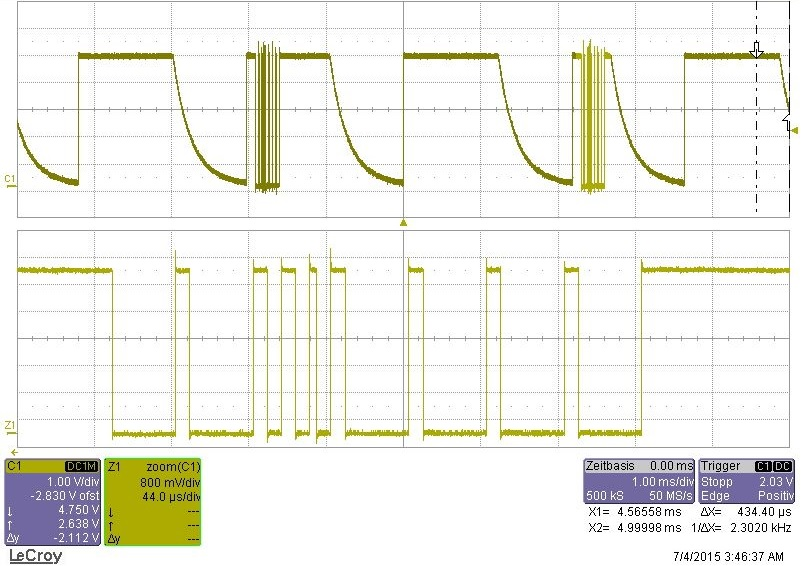
\includegraphics[scale=0.7]{chapters/userapplication/figures/DMX-Edge}
	\caption{DMX Protokoll: Problem fallende Flanke}
	\label{fig:DMX-Edge}
\end{figure}

\begin{figure}[H]
	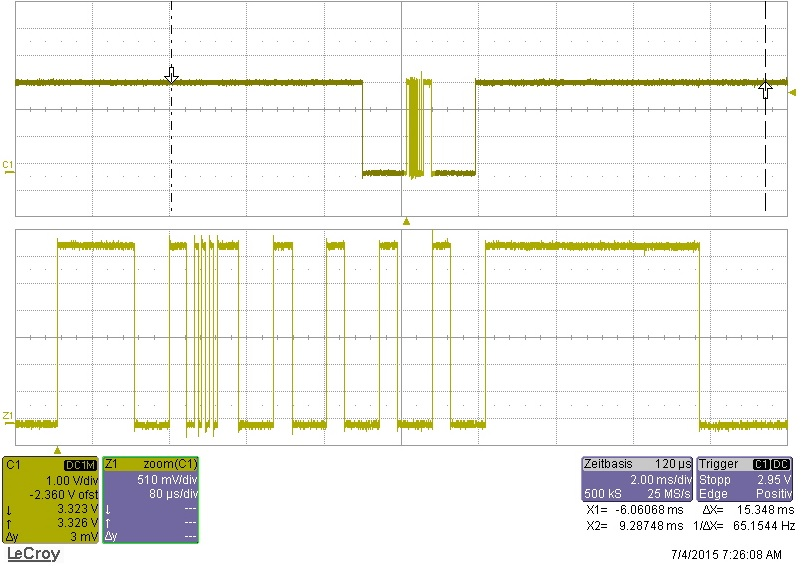
\includegraphics[scale=0.7]{chapters/userapplication/figures/DMX-Offset-Byte}
	\caption{DMX Protokoll: Problem Offset Byte}
	\label{fig:DMX-Offset-Byte}
\end{figure}

\begin{figure}[H]
	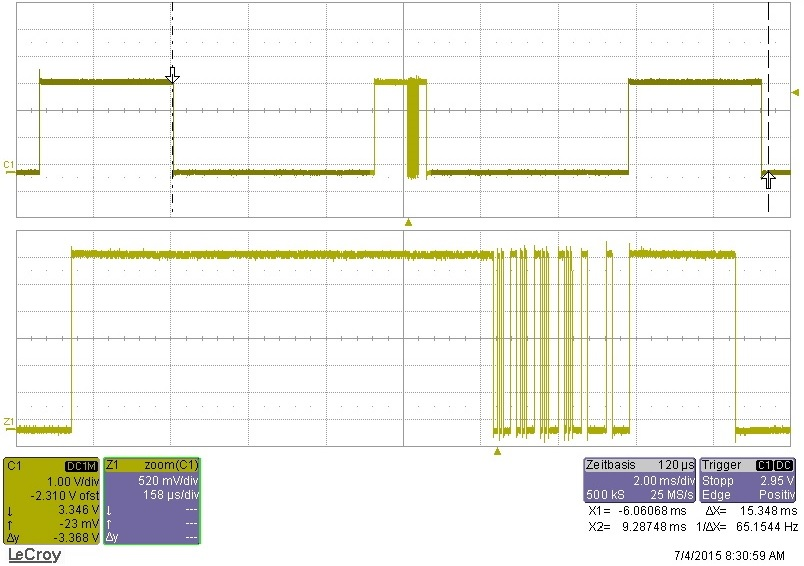
\includegraphics[scale=0.7]{chapters/userapplication/figures/DMX}
	\caption{Funktionierendes DMX Protokoll}
	\label{fig:DMX}
\end{figure}

\pagebreak 